\documentclass{sig-alternate}
\usepackage{amsmath}
\usepackage[T1]{fontenc}
\usepackage{ae, aecompl}
\usepackage{color}
%\usepackage{caption}
\usepackage{booktabs}
\usepackage{paralist}
\usepackage{graphicx}
\usepackage{amsfonts}
\usepackage{times}
\usepackage{cite}
\usepackage{float}
%\DeclareCaptionType{copyrightbox}
\usepackage[hyphens]{url}
\usepackage{enumerate}
\usepackage{algorithmicx}
\usepackage{algpseudocode}
\usepackage{algorithm}

\newcommand{\nn}{\nonumber}
\newcommand{\set}[1]{\mathcal{#1}}        			% Set
\newcommand{\rv}[1]{\boldsymbol{#1}}    			% Random variable
\renewcommand{\vec}[1]{\boldsymbol{\mathrm{#1}}} 	% Vector or Matrix
\newcommand{\event}[1]{\langle #1 \rangle}      	% Event
\newcommand{\arthur}[1]{\textcolor{blue}{Arthur: #1}}
\newcommand{\fixit}[1]{\textcolor{red}{#1}}
\newcommand{\etal}{\emph{et~al.}}


\renewcommand{\itemize}{\compactitem}
 \renewcommand{\enumerate}{\compactenum}

\newenvironment{mymathbox}
{\par\smallskip\centering\begin{lrbox}{0}%
\begin{minipage}[c]{0.8\textwidth}}
{\end{minipage}\end{lrbox}%
\framebox[0.9\textwidth]{\usebox{0}}%
\par\medskip
\ignorespacesafterend}
\begin{document}

%\title{Bitcoin Fraud with Targeted Blockchain Forks}
\title{Quantifying Web Adblocker Privacy}
%\title{Bitcoin Block and Transaction Withholding}
%\title{On Withholding Blocks and Transactions in Bitcoin}
%\title{Consequences of Withholding Blocks and Transactions in Bitcoin}
%\title{Consequences of Data Delivery Delay in Bitcoin}
%\title{Data Delivery Delay in Bitcoin}
%\numberofauthors{1}
%\author{}
%\numberofauthors{1}
%\author{Arthur Gervais$^\dag$, Hubert Ritzdorf$^\dag$, Ghassan O. Karame$^\dag$, Srdjan Capkun$^\dag$\\ \medskip \affaddr{$^\dag$ETH Zurich, Switzerland} \\ \email{$^\dag$firstname.lastname@inf.ethz.ch} }

\numberofauthors{1}
%\author{$^\dag$, $^\dag$, $^\ddag$ and $^\dag$\\ \medskip \affaddr{$^\dag$ETH Zurich, Switzerland \\ \email{$^\dag$firstname.lastname@inf.ethz.ch }

\maketitle

\begin{abstract}
\end{abstract}

\section{Introduction} \label{sec:introduction}

Advertising company models: direct buy, ad networks, ad exchanges.

\begin{itemize}
\item Adblocker - browser plugin blocking web advertisements
\end{itemize}


\section{Background} \label{sec:background}
The literature employed the number of blacklisted domains as a privacy indication~\cite{XX}, but we argue that this is not a sufficient indicator for the offered privacy enhancements. Instead of only capturing the reduction in percentage of accessed third parties, we argue that the graph of third parties should be analyzed in its entirety. Certain third parties are furthermore clearly collaborating, since they belong to the same logical entity. We therefore define the following privacy metrics in order to objectively compare different adblocker.

\section{Privacy metrics} \label{sec:background}
In this Section we introduce the privacy metrics used in order to quantify the privacy provisions of adblocker.

We model the tracking of a user $U$ through third parties as undirected graph $G=(E,V)$, where $E$ are edges, and $V$ vertices. A vertice can represent either a first party \emph{fp} (i.e. the URL the user visits) or a third party \emph{tp} (i.e. the URL of a resource that a first party fetches). An edge is built between a \emph{fp} that fetches a \emph{tp}. By visiting a series of websites $S_U = \{w_1, w_2, .. , w_n\}$, the complete tracking graph $G$ becomes apparent.

We augment \emph{G} by incorporating the logical relationship between third party domains. Two \emph{tp}, belonging to the same logical entity are thus combined into one vertice, resulting in a hierarchical graph. Figure~\ref{fig:graph} visualizes the different components of the build graph. Given \emph{G}, we evaluate the respective privacy provisions based on the following metrics.

\begin{figure}[htb!]
  \centering
  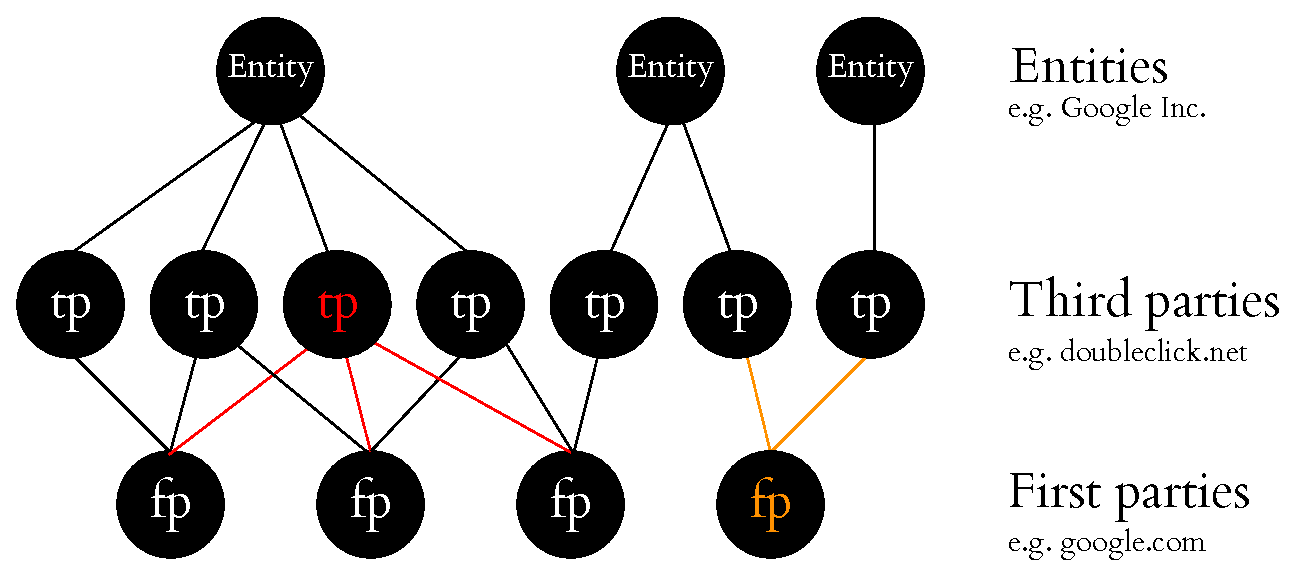
\includegraphics[width=0.45\textwidth]{figures/graph.eps}
  \caption{Graph built based on the regular crawling of the respective first parties. The colored third party has a node degree of 3, the colored first party has a node degree of 2.}\label{fig:graph}
\end{figure}

\paragraph{Add metric of how the BL changes (+ or - entries)}
\paragraph{Randomness of advertisement?}
\paragraph{Language extensions --> ghostery do we have the international profile?}

Crawl 5 times per day independently to quantify ad variance.

\paragraph{Degree of first party}
The more third parties a first party loads, the more likely the user is tracked. We therefore assess the number of edges of the first parties, equivalent to the degree of the first party vertices in graph $G$. By comparing the reduction in first parties with and without adblocker, we can objectively compare the improvement in the offered privacy of an adblocker.

\paragraph{Degree of third party}
The more often a third party is accessed over the users' series of websites $S_U$, the less privacy the user experiences from this particular third party. This intuition can be explained as follows. Let's assume that a third party is only loaded once from a first party in the series of websites $S_U$ loaded by $U$. This third party will learn that the user has accessed the respective first party, but has a limited view of the surf behavior of $U$. If the third party, however, is requested in over 80\% of the users' visited websites, the third party is likely to recover 80\% of the users' web behavior.

We capture this privacy notion, by assessing the degree of the third party nodes in the graph $G$ with respect to first parties. 
Similar to the degree of first parties, we can then evaluate the improvement in the offered privacy of an adblock software.

\paragraph{Graph density}
In addition the the outlined privacy metrics, we consider the graph density of $G$. The more dense $G$ is, the more third parties are likely to be able to track the user $U$. The graph density therefore allows to reason about the possible privacy improvements by the respective adblock software. For undirected graphs, the graph density is commonly defined as:
\begin{equation}
D = \frac{2 |E|}{|V|(|V|-1)}
\end{equation}

Note, that we cannot achieve the maximum density of 1, because the first parties are usually not directly connected.

\paragraph{Blacklist latency}
The formerly presented metrics only allow us to reason about the privacy provisions of the advertisement blocking software at a given time $t$. The advertisement industry, however, operates dynamically by using e.g., new advertisement techniques and new third party URLs. In order to capture the temporal privacy provisions of the adblocker, we evaluate the the aforementioned privacy metrics over a timespan of several months. This allows us to reason quantitatively about how fast an adblocker adapts to a changing advertisement environment.

\subsection{Beyond URLs}
The presented metrics capture the raw third party URLs. Since the URL information, however, does not capture many aspects of the respective web infrastructure and resulting privacy risks, we augment the graph $G$, by incorporating, logical entities, cookies, and if a third party contains active or passive content.

\paragraph{Logical entity}
Instead of focusing on the URL of a third party, we link the third parties based on their respective owner information. Third parties such as \url{doubleclick.net} and \url{google.com} for example are both owned by the same entity Google Inc. Their collusion therefore seems more likely, and affects the privacy of a web user $U$ more significantly, than if both were belonging to two different logical entities. By incorporating the logical relation among third party domains, we therefore capture a more realistic privacy leakage through user web surf activity.

\paragraph{Cookies}
Capture if a third party sets a cookie

\paragraph{Active vs. static content}
Active content is more critical than static

\paragraph{DNT influence}
Does DNT change something (has been studied before).

\section{Evaluation}

\subsection{Experimental setup}

\subsubsection{Lightbeam first party heuristic}

\subsection{Blocked pure third parties}

\paragraph{Degree of first party}
\begin{figure}[h]
  \centering
  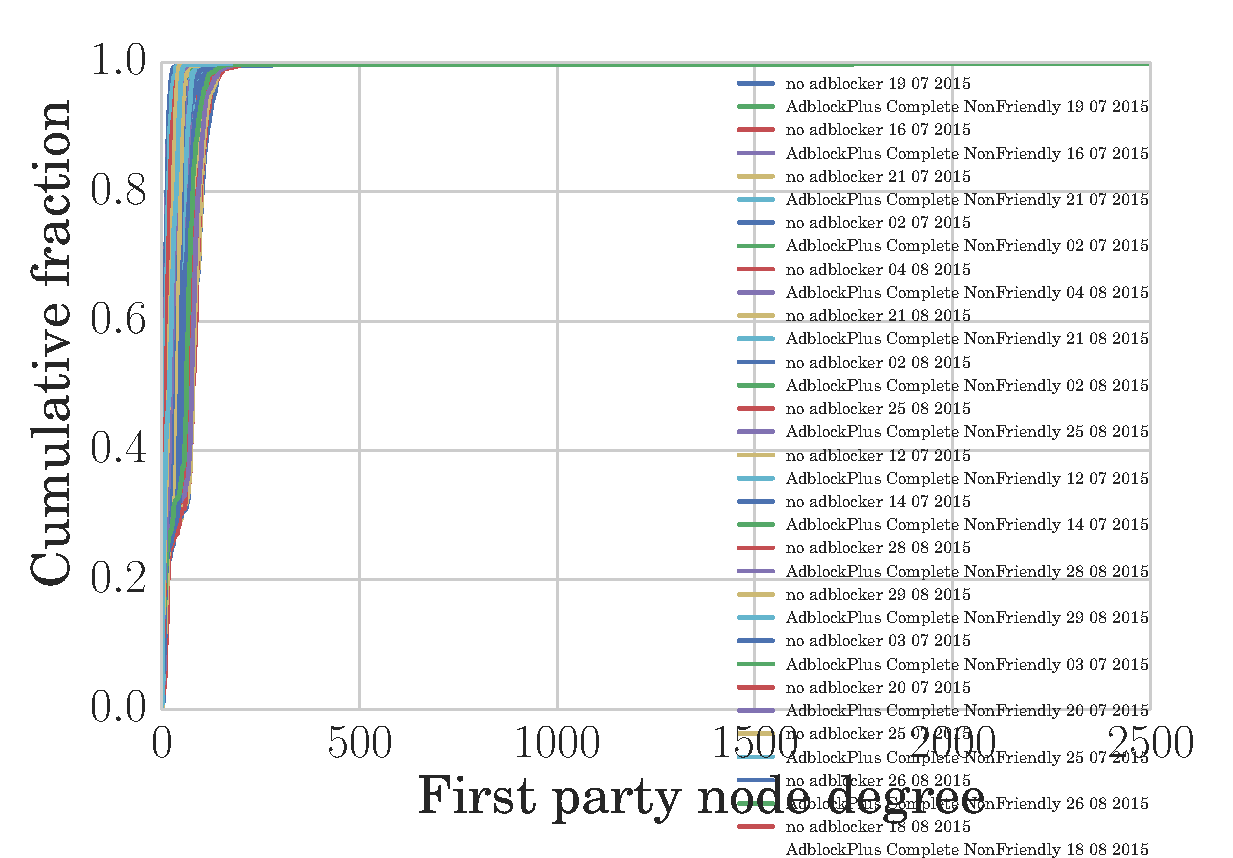
\includegraphics[width=0.45\textwidth]{figures/degree_first_parties.eps}
  \caption{Degree of first party nodes in the resulting graph of the respective adblock software. Intuitively, in the case of no adblocker, the first party degrees are highest.}\label{fig:degree_first_parties}
\end{figure}
\paragraph{Degree of third party}
\begin{figure}[h]
  \centering
  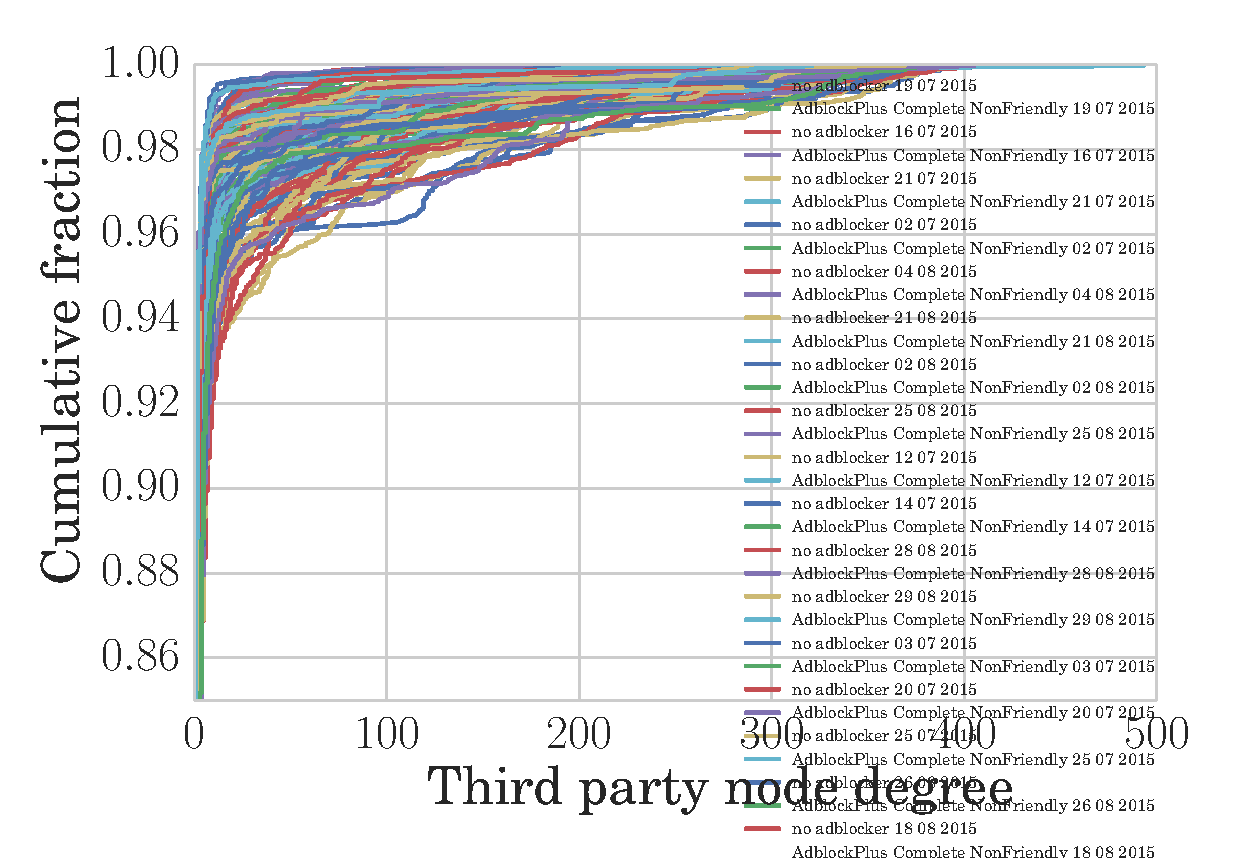
\includegraphics[width=0.45\textwidth]{figures/degree_third_parties.eps}
  \caption{Degree of third party nodes in the resulting graph of the respective adblock software. Intuitively, in the case of no adblocker, the third party degrees are highest.}\label{fig:degree_third_parties}
\end{figure}
\paragraph{Graph density}

\begin{table}[htb!]
\centering
\begin{tabular}{l l }
\toprule
Adblocker & Graph density\\
\midrule
No adblocker & 0.00296\\
Adblock & 0.00268\\
Ghostery & 0.00201\\
\bottomrule
\end{tabular}
\caption{Graph density of the respective adblocker. Intuitively, if no adblock software present, the graph density is at it's maximum.}\label{tb:graph_density}
\end{table}

\subsection{Blocked logical third parties}
\subsection{DNT influence}
See if DNT has an influence on the number of third party changes
\subsection{Blacklist latency}

\subsection{Practical considerations}
\begin{itemize}
	\item Network Prediction services should be disabled (e.g. Chrome offers this option.) if these requests are not captured by the adblocker.
\end{itemize}

\section{Related work}
NSDI 2013 Google, alexis
https://cyberlaw.stanford.edu/files/publication/files/trackingsurvey12.pdf
Advertisement bidding
ublock.org is a lightweight blocking proxy
https://trackography.org/

\section{Conclusions} \label{sec:conclusions}

\bibliographystyle{plain}
\bibliography{relatedwork}
\end{document}
